%%==================================================
%% chapter02.tex for BIT Master Thesis
%% modified by yang yating
%% version: 0.1
%% last update: Dec 25th, 2016
%%==================================================
\chapter{多维源代码表征学习方法总体设计}

本章首先介绍代码表征学习面临的一些关键技术挑战,基于此提出本文的面向代码克隆检测的多维源代码表征方法框架RLCCD的研究方案,并就该框架的设计思路和总体架构进行详细阐述。此外也简要介绍了该框架包含的3个流程,即代码预处理、多维源代码表征学习、克隆检测任务实现。

\section{代码表征学习关键技术挑战}
\label{challenges}

目前已有的代码克隆检测方法大多遵循以下思路:(1)首先对代码片段进行预处理;(2)对处理好的代码片段进行信息抽取,将其转换为中间表征;(3)根据表征的方式不同计算不同代码片段之间的相似度,完成克隆检测任务。


代码表征学习的技术难题

(1)Token:集外词问题

(2)AST:树高度过深导致梯度消失问题

(3)PDG:图算法开销大问题


\section{RLCCD框架研究方案}
针对上述提出的技术中面临的关键挑战,本文提出面向代码克隆检测的多维源代码表征方法RLCCD。本节首先介绍RLCCD框架的研究思路及总体框架,然后根据流程介绍代码处理、多维源代码表征学习、克隆检测任务实现三个步骤,其中,多维源代码表征学习步骤中分别针对\ref{challenges}节提出的3个关键挑战提出了对应的解决办法。

\subsection{研究思路及总体框架}

基于上述研究思路,本文提出的自适应潜力感知模糊测试技术框架如图\ref{fig:framework}所示,由图可见,本文提出的基本框架与代码克隆检测的处理流程基本一致,并主要通过三个维度对代码表征环节进行优化。

\begin{figure}[H]
    \centering
    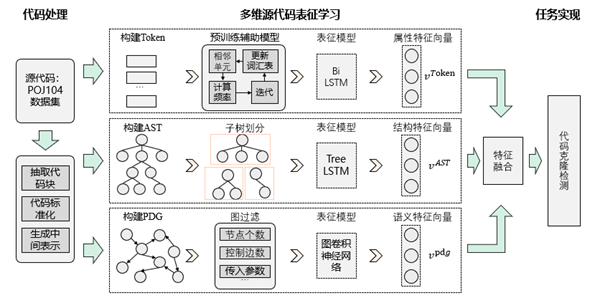
\includegraphics[width=0.95\textwidth]{figures/framework}
    \caption{RLCCD 总体框架}
    \label{fig:framework}
\end{figure}

下面则分别对代码处理、多维源代码表征学习、克隆检测任务实现的流程和关键技术点进行介绍。

\subsection{代码处理}
代码处理的目标是生成源代码片段对应的Token序列、抽象语法树和程序依赖图,主要包含3个流程:抽取代码块、代码标准化、生成中间表示。首先,使用TXL工具从源代码中提取出代码块。这里的源码来自POJ104公共数据基准集,而TXL是专门为软件分析和源代码转换任务设计的一个分析工具,可以很好地支持C语言;然后,对代码块中的代码进行代码标准化处理。具体的,首先需要去除代码块中的注释、空格和空行,然后根据一定的转化规则进行代码标准化;最后,基于标准化后的代码片段生成对应的中间表示:Token序列、抽象语法树AST和程序依赖图PDG。

\subsection{多维源代码表征学习}
RLCCD框架的核心步骤是源代码表征学习,其目标是学习能够表示代码片段的连续向量,表现程序理解的认知层次,获取程序的语法、语义信息,创建程序更高抽象层次上的表示,它决定着对源代码信息抽取程度的上限,决定着检测方法的预处理方式、模型设计、部署方式、运行效率,并影响后续代码克隆检测任务所能检测的精度。下面从Token序列、抽象语法树AST、程序依赖图PDG三种不同维度的代码特征表示出发,详细介绍研究方案并分析其优化改进。

(1)针对Token序列特征挖掘,提出预训练增强辅助模型提取属性特征,从而解决传统基于Token序列的方法存在的集外词问题;

(2)针对抽象语法树AST特征挖掘,提出子树划分的改进方法提取结构特征,从而解决传统基于抽象语法树的方法存在的梯度消失问题;

(3)针对程序依赖图PDG特征挖掘,提出过滤机制提取语义特征,通过收集PDG的简单特征来过滤掉明显不可能为克隆的PDG对,从而解决传统基于程序依赖图的方法存在的计算开销大问题。

(4)特征融合方法
特征融合的目标是将提取到的属性特性、结构特征、语义特征合并,得到一个更能代表代码信息的多维特征,更具有判别能力。

按照具体的技术,特征融合包括特征拼接、特征求和(均值、pooling、加权求和)、特征之间对应元素相乘、特征之间求外积再送入神经网络、跳跃连接(skip)、反卷积、典型相关分析CCA、注意力机制(包括self-attention)加权求和、构图然后采用图神经网络等等。

\subsection{克隆检测任务实现}
克隆检测任务实现的目标是通过计算两个代码的向量距离来判断是否存在代码克隆。常见的向量距离包括欧式距离、曼哈顿距离等。由于代码克隆检测问题是一个二分类问题,即给定两个代码片段,需要输出0或1,0表示它们之间不相似,1表示相似。因此需要将向量距离d映射到0~1之间,这里可以通过sigmoid函数、tanh函数等做映射,其函数值表示两个代码片段的相似度。然后设定阈值,当相似度大于阈值,则判定两个代码片段属于代码克隆,输出1。

\section{本章小结}
本章首先分析了源代码表征学习在代码克隆检测过程中所面临的关键技术挑战,主要表现为Token集外词问题、树梯度消失问题、图计算开销大问题。针对上述提出的三个问题,提出了本文的方法RLCCD,并介绍了其整体框架和处理流程,对其中的关键技术点进行了简要的论述。



